\documentclass[11pt]{article}
\usepackage[a4paper,margin=2.2cm]{geometry}
\usepackage{amsmath,amssymb}
\usepackage{booktabs}
\usepackage{array}
\usepackage{enumitem}
\usepackage{xcolor}
\usepackage{tikz}
\usepackage{caption}
\usetikzlibrary{arrows.meta,positioning,shapes.geometric}
\usepackage[hidelinks]{hyperref}
\newcommand{\code}[1]{\texttt{\small #1}}
\newcommand{\meas}{\textcolor{green!50!black}{\textbf{MEASURED}}}
\newcommand{\hyp}{\textcolor{orange!80!black}{\textbf{HYPOTHESIS}}}
\tikzset{
  box/.style ={draw, rounded corners, align=center, font=\small, fill=blue!4, minimum height=8mm},
  dec/.style ={draw, diamond, aspect=2.2, align=center, font=\scriptsize, fill=yellow!12, inner sep=1pt},
  good/.style={draw, rounded corners, align=center, font=\small, fill=green!8, minimum height=8mm},
  back/.style={draw, rounded corners, align=center, font=\small, fill=red!5, dashed, very thick, draw=red!55, minimum height=8mm},
  arr/.style ={-{Stealth[length=2.2mm]}, thick},
}
\title{\textbf{Geometry-native primitive replacement}\\[2pt]
  \large A parity-gated design principle (measurement-grounded, fallback-mandatory)}
\author{Dr.\ Csaba Hajdu}
\date{2026-06-22}
\begin{document}\maketitle

\noindent\textbf{The principle.} Across the framework, prefer \emph{learnable, geometry-/structure-native}
primitives over fixed black-box ones --- \code{tanh}$\to$ Catmull-Rom (CR) spline, plain aggregation $\to$
signed rotor propagation, node-ID table $\to$ signed structural features, \code{softmax}$\to$ rotor scoring.
\textbf{But} (the two binding conditions): a native primitive becomes the default \emph{only} after a
parameter-matched ablation shows \textbf{$\ge$ parity by measurement}, and the legacy primitive is \textbf{always
retained as a config-axis fallback}. The justification for the swap is \emph{consistency / boundedness /
quantization / hardware fit / auditability} --- \textbf{not} a claimed accuracy gain, because the fair ablations
to date show parity (and one readout case where the simple op wins).

\section*{The decision gate (every swap)}
\begin{center}
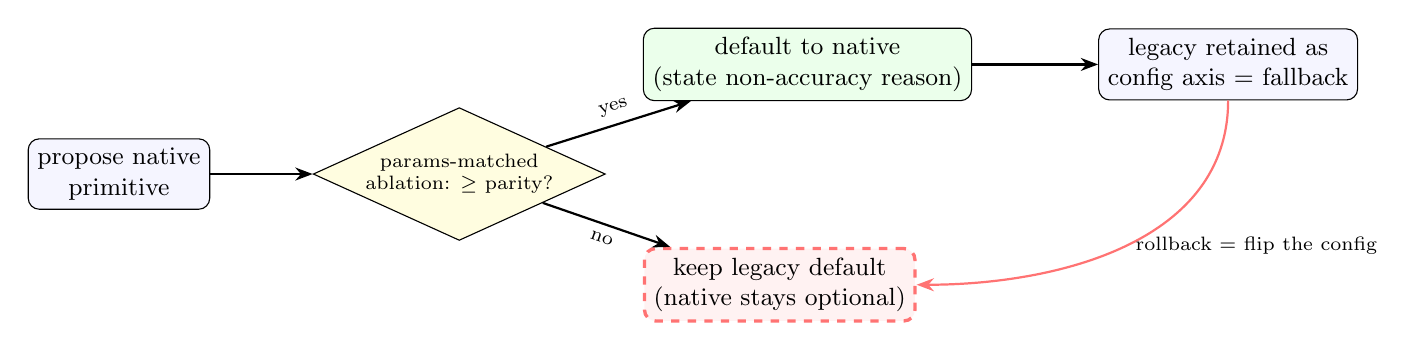
\begin{tikzpicture}[node distance=7mm and 13mm]
  \node[box] (prop) {propose native\\primitive};
  \node[dec, right=of prop] (gate) {params-matched\\ablation: $\ge$ parity?};
  \node[good, above right=5mm and 14mm of gate] (def) {default to native\\(state non-accuracy reason)};
  \node[back, below right=5mm and 14mm of gate] (keep) {keep legacy default\\(native stays optional)};
  \node[box, right=16mm of def] (fb) {legacy retained as\\config axis = fallback};
  \draw[arr] (prop)--(gate);
  \draw[arr] (gate)-- node[above,sloped,font=\scriptsize]{yes} (def);
  \draw[arr] (gate)-- node[below,sloped,font=\scriptsize]{no} (keep);
  \draw[arr] (def)--(fb);
  \draw[arr, draw=red!55] (fb.south) to[out=-90,in=0] node[right,font=\scriptsize]{rollback = flip the config} (keep.east);
\end{tikzpicture}
\end{center}

\section*{The ledger (what is measured, what is still a bet)}
\renewcommand{\arraystretch}{1.25}
\begin{center}\small
\begin{tabular}{>{\raggedright\arraybackslash}p{0.20\textwidth} >{\raggedright\arraybackslash}p{0.21\textwidth} l >{\raggedright\arraybackslash}p{0.34\textwidth}}
\toprule
swap & status & & evidence / fallback \\
\midrule
edge activation \code{tanh}$\to$\,CR spline & \emph{parity} on accuracy & \meas &
  toy non-monotone probe, 3-seed: cr$\approx$tanh at matched params; a wider tanh edges ahead \emph{per param}
  $\Rightarrow$ no accuracy buy. RL test = the campaign. \textbf{fallback} \code{activation$\in$\{cr,tanh\}} \\
propagation $\to$ signed rotor slerp/nlerp & first confirmed \emph{lift} & \meas &
  +0.0045 alpha / +0.0105 otc, 5-seed, leakage-clean (\code{2026-06-17-signed-rotor-slerp-propagation}); \textbf{fallback} propagation off \\
embedding geometry: rotor S$^3$ vs MLP-embed & \emph{parity}, not load-bearing & \meas &
  $\pm$0.002--0.005, inside $\sigma$ (\code{2026-06-18-rotor-vs-mlp-embed-ablation}); \textbf{fallback} MLP-embed \\
\textbf{readout head} geometric vs real bilinear & legacy \emph{wins} (boundary!) & \meas &
  complex/quaternion/geodesic \emph{worse} (\code{2026-06-17-link-head-ablation}); \textbf{do not} geometric-ise the output \\
attention \code{softmax}$\to$ rotor scoring & parity-likely; benefit off-manifold & \hyp &
  rotor "doesn't kill performance" generalised from above; \textbf{fallback} \code{score$\in$\{softmax,rotor\}}, gate first \\
control backbone MLP$\to$HSiKAN & parity so far & \meas/\hyp &
  cart-pole + Galambos single-seed tie; multi-seed in flight; \textbf{fallback} \code{kind$\in$\{mlp,hsikan\}} \\
rotor output $\to$ int8 quantization (Nagare) & calibration-free quantize & \hyp &
  bounded S$^3$ output; the \emph{discriminator} is planned, not run (\code{2026-06-18-rotor-embedded-nagare}) \\
\bottomrule
\end{tabular}
\end{center}

\section*{The rules (binding)}
\begin{enumerate}[nosep, leftmargin=1.5em]
  \item \textbf{Measured parity gate.} No native primitive becomes the default without a params-matched
        ablation showing $\ge$ parity (median gap within cross-seed IQR). Until then it ships \emph{off by
        default}, available behind its config axis. ``Rotor didn't hurt once'' is a datapoint, not a licence.
  \item \textbf{Mandatory fallback.} Every swap is a \emph{config axis} that retains the legacy primitive
        (\code{activation$\in$\{cr,tanh\}}, \code{score$\in$\{softmax,rotor\}}, \code{kind$\in$\{mlp,hsikan\}}).
        Rollback is flipping the flag --- no code change, no migration.
  \item \textbf{Honest justification.} State the reason as consistency / boundedness / quantization / hardware /
        auditability. Do \emph{not} claim accuracy; the fair ablations show parity, and the \emph{readout} is a
        measured counter-example where the simple op wins --- a hard boundary of the principle.
  \item \textbf{Distinguish in writing} what is measured from what is a hypothesis (this ledger), and run the
        discriminating ablation before promoting a hypothesis row to a default.
\end{enumerate}

\noindent\textit{Status note:} the CR activation swap (\code{hymeko\_rl/policy.py}) + its
\code{activation$\in$\{cr,tanh\}} fallback are implemented and \textbf{verified} (15 policy tests incl.\ a
parity test vs \code{signedkan\_wip}). The toy A/B above shows \textbf{accuracy parity}, so CR ships as the
default on the \emph{consistency/KAN-structure} rationale --- not an accuracy claim --- exactly per this
principle. The real-topology RL read is the in-flight CR campaign.

\end{document}
